\documentclass[11pt,english,twocolumn]{article}

\usepackage{graphicx}
\usepackage{subfigure}

\title{Append-only Datastore}
\author{
	Mingyan Zhao \\
    myzh@stanford.edu
	\and
	Steven Tung\\
    steven.tung@stanford.edu
	\and
	Kevin Krakauer\\
    kevinkrakauer@gmail.com
}
\date{}

\begin{document}

\maketitle

% Calling our operation "put" is inherently confusing, I'm using "append".

\section*{Abstract}
We built an eventually consistent, append-only datastore focused on low
read/write latency and high availability. In the common case, clients interact
only with nearby nodes for extremely low latency. Data is always appended to the 
store for a given key and the relative order of observed data is maintained.

The datastore is eventually consistent. Data is stored in memory for low latency
and in local disk for safety. Nodes can operate when disconnected from the
system, preserving availability in the face of total and long-term partitioning.
We believe this system will be useful in chat, social media, and distributed
logging applications.

\vspace{-0.4cm}
\section{Introduction}
\vspace{-0.2cm}
As organizations increasingly move to the cloud, applications are designed from
the ground up with a distributed architecture (\textit{microservices}). Despite
numerous advantages, distributed application design requires addressing latency
and partitioning concerns that monolithic applications do not have.

Our \textit{append-only datastore} addresses latency and partitioning concerns
for append-only workloads. It is designed to run as a service distributed
globally across multiple data centers. By explicitly distinguishing between a
\textit{leader} node and \textit{follower} nodes, we gain several advantages
over other eventually consistent systems:
\begin{enumerate}
	\item Clients communicate only with their nearest follower for extremely
		low latency. \vspace{-0.3cm}
	\item Eventual consistency is minimally disruptive to clients. A client
		may read the data for key $k$ and receive data consisting of 2
		writes' data: $\{d_1, d_2\}$. Write $x$ with data $d_x$ sent
		through another follower preserves the ordering of $d_1$ and
		$d_2$, so the system eventually returns $\{d_x, d_1, d_2\}$,
		$\{d_1, d_x, d_2\}$, or $\{d_1, d_2, d_x\}$ when read.
\end{enumerate}
We also gain the advantages of some more traditionally eventually consistent
systems, such as great partition tolerance \cite{Dynamo}. Together, these
properties are highly desirable for many append-only applications. Consider the
following:

\begin{itemize}
	\item \textbf{Distributed logging} - Consider a monitoring service using
		the append-only datastore for logs in real time. The service
		writes and retrieves logs with extremely low latency from the
		nearby data center. Also it is provided an eventually consistent
		log that contains data from all of the deployments.
	\item \textbf{Chat Application} - Consider a chatroom
		occupied by a team in North America and a team in Asia. Each
		team member sees their local peers' messages immediately, and
		all messages eventually.
\end{itemize}

\section{Related Work}
Amazon's Dynamo \cite{Dynamo} supports always-writable semantics, high partition
tolerance, and laser-focuses on low-latency operation. Unlike our system, Dynamo
is a key-value store. It also exposes a great deal of complexity to developers,
who must tailor their use of Dynamo such that conflicts are resolvable and
must manually implement conflict resolution in clients. Our system does not
allow for conflicts. Google's GFS \cite{GFS} is also optimized for append-heavy workloads and uses a
single master for simplicity and intelligent coordination. It supports random
writes as well. However, it is explicitly optimized for non-latency-sensitive
applications, and a single read can require multiple hops (the GFS master and
chunkserver). LinkedIn's Kafka \cite{Kafka} provides eventual delivery of large
quantities of data, but running under a publish/subscribe
mechanism.

\vspace{-0.4cm}
\section{Design}
Nodes in the append-only datastore are classified in a simple hierarchy as seen
in Figure \ref{Architecture}. A single \textit{leader} directs multiple
\textit{followers}. Clients connect to and communicate with a nearby follower,
likely running in the same data center, to minimize latency. Our design tolerates
arbitrary partitions between nodes and ensures an eventually consistent view of
data.
%\vspace{-0.4cm}
% Architecture
\begin{figure}[t]
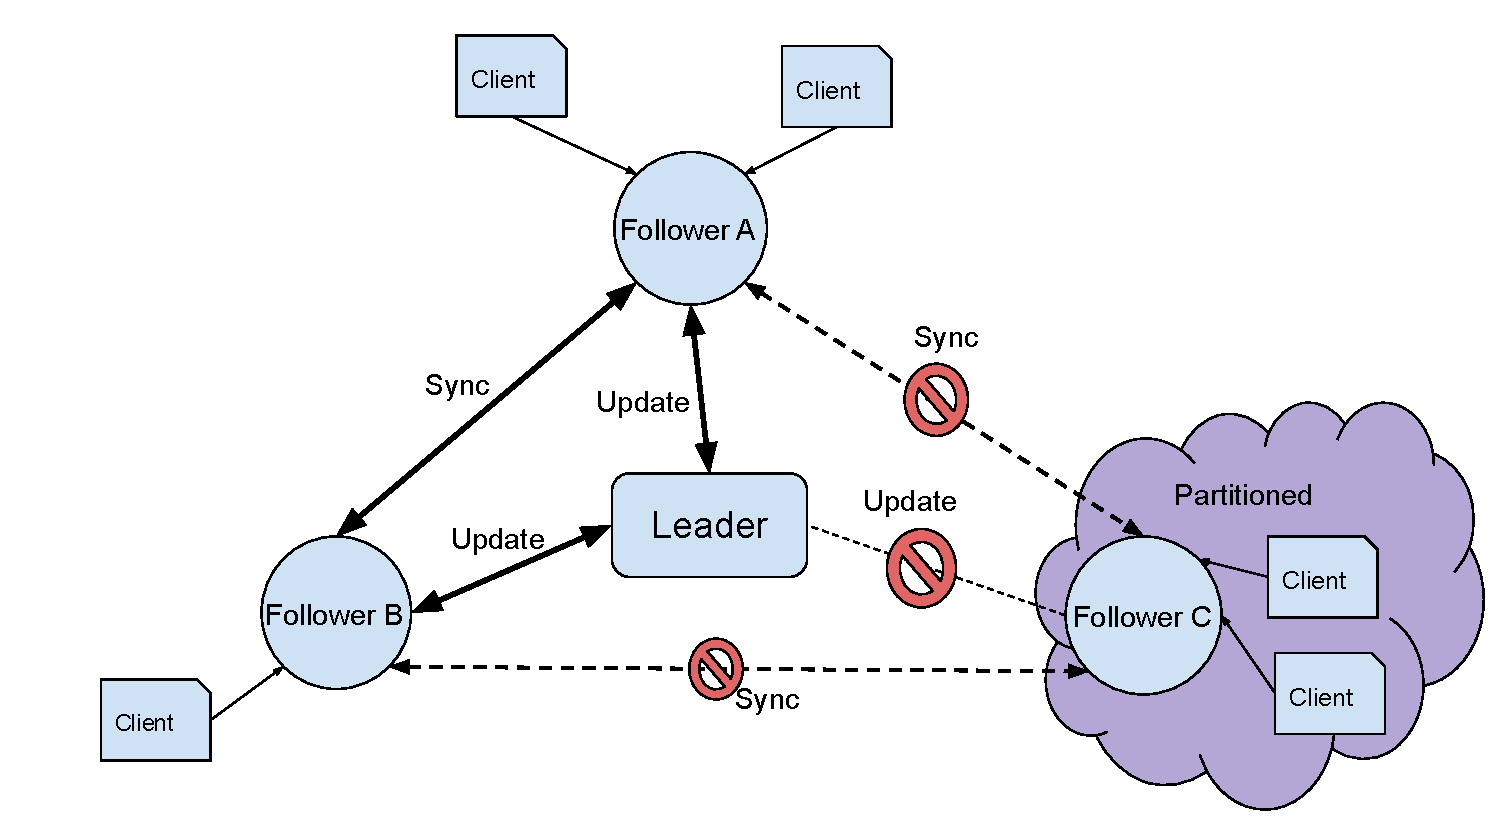
\includegraphics[width=8cm]{figure/SystemStructure.pdf}
\caption{Architecture}
\label{Architecture}
\end{figure}
Clients are exposed to the following API by followers:
\begin{itemize}
	\item \texttt{append(key, data)} - Appends \texttt{data} to the existing
		data for \texttt{key}. Guarantees that \texttt{data} will be
		committed eventually if it is written to local disk.
	\item \texttt{get(key)} - Gets the data for \texttt{key}, represented as a
		list of values. Later calls to \texttt{get} return data in the
		same relative order, but other data may be interleaved or
		appended.
\end{itemize}

\subsection{Leader}
% TODO: Explain what happens when this is partitioned. Look at gfs paper.
The leader is responsible for globally ordering writes for each key. Like GFS's
master \cite{GFS}, it only stores metadata rather than the value itself.
This decreases network usage.  Also, the
burden on disks is lighter per update, increasing writes per second and the
average lifetime of each disk. The simplicity of a single master
simplifies our implementation and the rest of our design, which increases
the overall stability of the system. 

\subsubsection{Index number}
The leader maintains the latest index number for all keys. Index numbers are
globally unique and monotonically increasing. Once generated, each is mapped
to a list of values on the requesting follower. If another follower needs that
value, it simply needs the index number to fetch the data.

\vspace{-0.4cm}
\subsubsection{Update}
Upon receiving an \texttt{Update} request, the leader advances the index
number by one and updates the follower information to the incoming one.

The \texttt{Leader} decides whether the requesting follower needs to sync up
with other followers. If a mapping exists from key $k$ to index $i$, an
\texttt{Update} carrying the same index $i$ does not need a Sync ($i$ still
increments by 1). This may happen when 1) a key created on the leader for the
first time, or 2) the requesting follower is the same as the recorded follower
for the key.

An \texttt{Update} to $i' < i$ indicates that the sender does not have the
latest data. In this case the leader signals the follower to sync with the
follower in its records that originated the append at index $i$. This may happen
when two followers are append data to the same key concurrently. The common,
non-concurrent case is shown in Figure \ref{CommonUpdate}.

% update procedure figure
\begin{figure}[h]
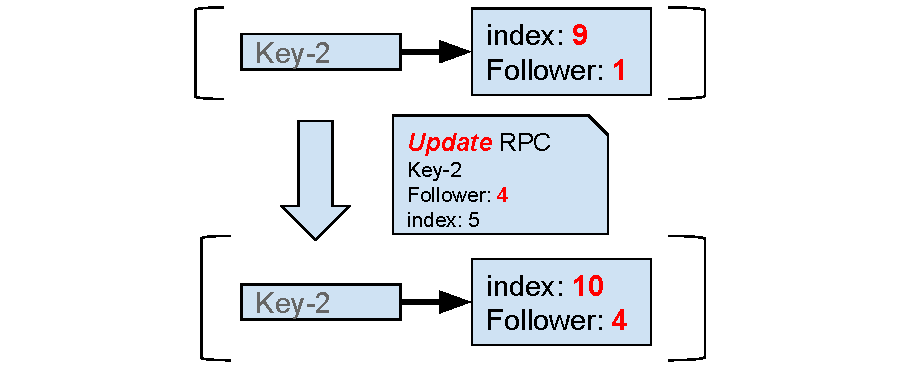
\includegraphics[width=8cm]{figure/update.pdf}
\caption{Update procedure}
\label{CommonUpdate}
\end{figure}

\vspace{-0.3cm}
\subsubsection{Broadcasting index numbers}
The leader broadcasts ensure the eventual consistency of the system. Each
appended value gets replicated and synced immediately between the requesting
followers and in-record follower, but all of the other followers do not know
it until the leader broadcasts the latest index number. 

Depending on the workload and use cases, we provide different ways of
broadcasting. One is triggered per-request, which is expected to provide lower
consistency latency but may only be used in a lower QPS scenario, since the
broadcasting may cause a great amount of communication between the followers.
The other one is triggered periodically, which is expected to be used in most
cases. The leader broadcasts the updated keys and their index numbers repeatedly
at a small, set interval.

\subsubsection{Leader Fault Tolerance}
Because the leader writes all updates to disk, it tolerates crashes and reboots.
For greater fault tolerance, it should write to multiple disks or a remote disk
as well.

The system continues to function when the leader is partitioned, but followers
and thus clients do not receive updates from other followers. As long as the
partition is eventually healed, the system will propagate information correctly
and self-heal. If for some reason there is a permanent partition, it must be
manually worked around by changing the cluster configuration (i.e. the set of
nodes in the system).

\subsection{Follower}
% Explain what happens when this is partitioned.
% Explain read-your-own-writes consistency.
% Be sure to discuss any synchronization that happens here, as the follower is
% responsible for synchronizing its the writes to it.
The follower is our most critical component. Its responsibilities include:

\begin{itemize}
	\item Handing \texttt{append} and \texttt{get} requests. \vspace{-0.4cm}
	\item Managing data. \vspace{-0.4cm}
	\item Updating the leader about appended data. \vspace{-0.4cm}
	\item Syncing with other followers to communicate updates and orderings.
\end{itemize}

\subsubsection{Data structure}
Followers replicate the entire datastore in memory to minimize
reading and writing latency. The data structure is described in Figure \ref{DataStructure}.

% data structure figure
\begin{figure}[h]
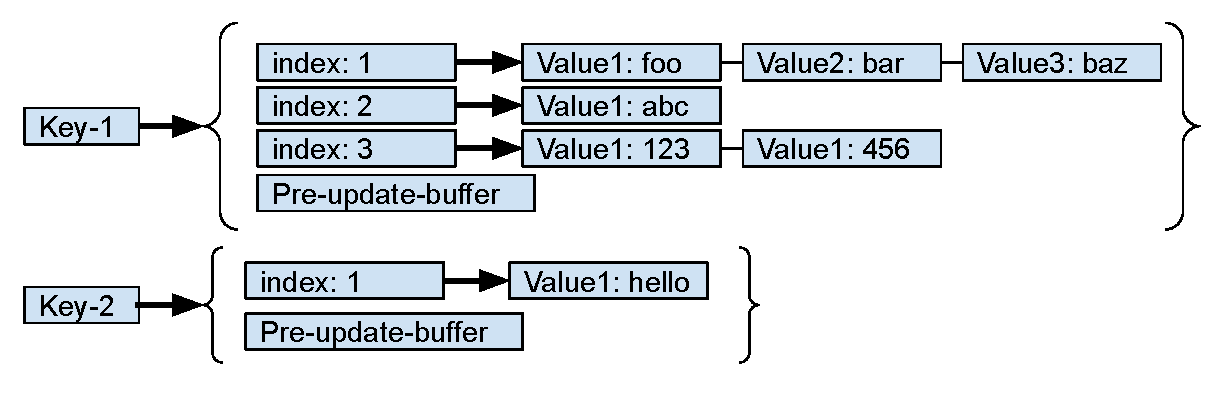
\includegraphics[width=8cm]{figure/DataStructure.pdf}
\caption{Data procedure on Follower}
\label{DataStructure}
\end{figure}

\subsubsection{Client Interfaces}
\textbf{Append(key, data):} Upon reviving an \texttt{Append} request, the
follower writes the data to memory first and then writes to a local disk for data
safety. It returns immediately after the data is written to local disk. For
increased fault tolerance, the append should be written to multiple disks
locally or to a remote disk. Note that throughout this section when we
refer to updating local storage, the in-memory store is also updated immediately
after data is written to disk.

The follower always appends data to the pre-update-buffer first, then issues an
\texttt{Update} if the pre-update-buffer is not empty. If it receives an
\texttt{Update} response with a index number, it creates a new index entry and
moves all of the data from pre-update-buffer to the new entry. 

\noindent \textbf{Get(key):} When clients issue a \texttt{Get} request, they are
served from the in-memory datastore. We guarantees that the data read by the
clients are correct, but not necessarily yet globally consistent. The follower
builds up a list with all of the data from each index as well as everything from
the pre-update-buffer.

\subsubsection{Synchronization}
Followers use the \texttt{Sync} request to get data they missed. This ensures
the eventual consistency of the system. \texttt{Sync} requests also signal what
data the sender has to the recipient, enabling the recipient to create new index
entries in its local datastore. The \texttt{Sync} request is issued when a
follower receives an \texttt{Update} response from the leader indicating it
needs synchronization. 

Since a follower may missing multiple indices of data, a \texttt{Sync} request
may carry a list of indices that it is asking for. However the recipient may
also be missing some of the indices if there is a large amount of \texttt{Sync}
requests in flight simultaneously. To mitigate this, the \texttt{Sync} response
only replies with indices and data the recipient already has, so that the
issuer can accept what is returned and do another \texttt{Sync} asking for
what is left. Eventually, each follower synchronizes with and achieves global
consistency.

Combined with the \texttt{Update} requests, Figure \ref{UpdateAndSync}
demonstrates a message flow of synchronization in common case.

% UpdateAndSync figure
\begin{figure}[h]
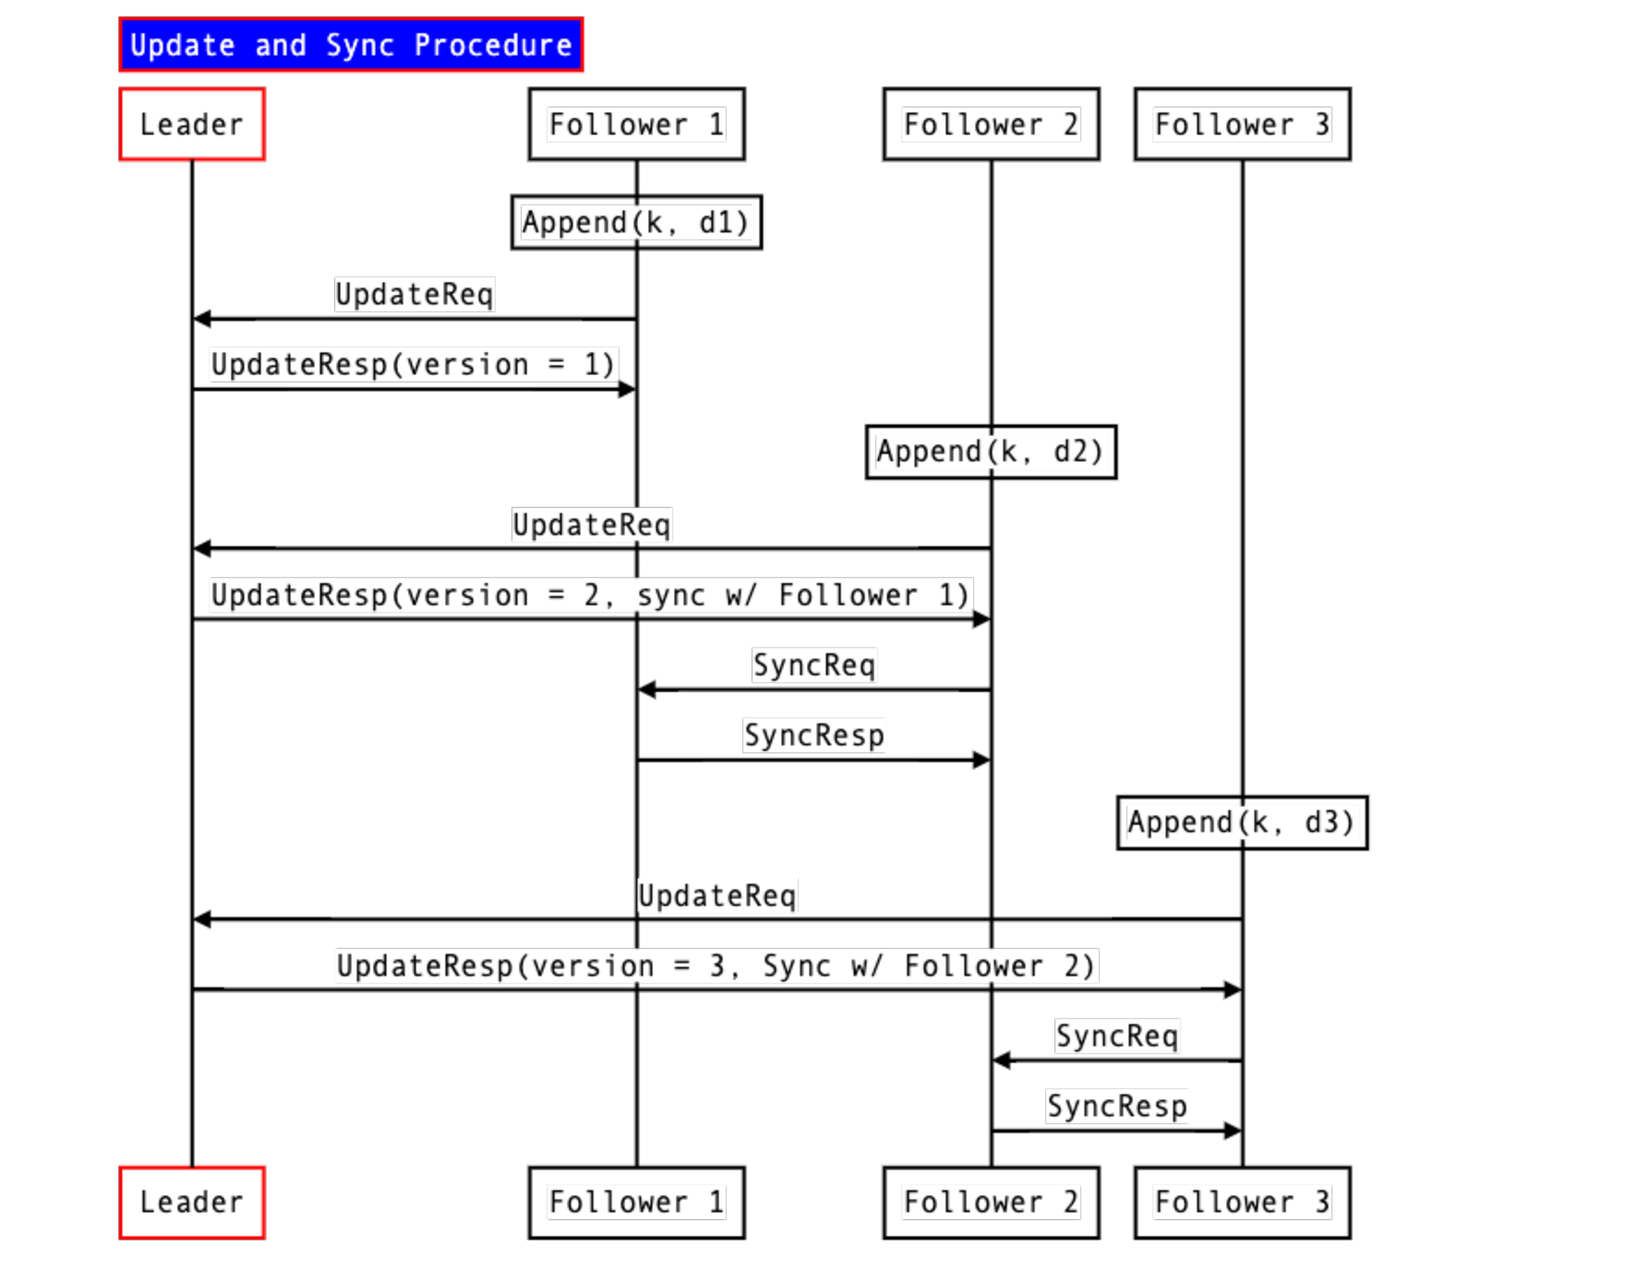
\includegraphics[width=8cm]{figure/UpdateAndSync.pdf}
\caption{Update and Sync message flow}
\label{UpdateAndSync}
\end{figure}

\subsubsection{Follower Fault Tolerance}
Both \texttt{Update} and \texttt{Sync} requests are retried in case of network
failure. If a follower reboots during a \texttt{update}, it can inspect the disk
at boot and see that it has appended data locally that has not been confirmed by
the leader. If a follower reboots during a \texttt{sync}, it will have stale
data until a \texttt{get} or \texttt{append} causes it to update. This keeps the
system simple while retaining its consistency properties.

\vspace{-0.4cm}
\section{Evaluation}
The system is written in Go and can be run manually or distributed and
run with Docker. Nodes communicate via gRPC. 

We ran tests with a cluster of Google Compute Engine virtual machines. Google
Cloud platform provides internal IP communication between VM instances, which
means request between servers do not go through the public Internet and are thus
fast. We deployed our system in the following locations.
\begin{itemize}
    \vspace{-0.4cm}
	\item One leader in Iowa, Central USA.
	\vspace{-0.4cm}
	\item One follower and one client in each of the following five locations
\vspace{-0.3cm}
    \begin{itemize}
    \item Iowa, central USA.
\vspace{-0.3cm}
	\item Los Angeles, west USA.
\vspace{-0.3cm}
	\item South Carolina, east USA.
\vspace{-0.3cm}
    \item London, west Europe.
\vspace{-0.3cm}
    \item Tokyo, northeast Asia.
\vspace{-0.3cm}
    \end{itemize}
\end{itemize}

In the performance test, each client in the performance test sends 120,000
\texttt{Append} against 10 keys randomly, so that in total there are
600,000 values in the datastore globally. After all of the \texttt{Appends} are
done, each client then retrieves the data by issuing \texttt{Get} for all of the
10 keys every 0.5 second periodically.

\subsection{Append Request Performance} We measures the \texttt{Append} request
latency in Table \ref{AppendLatency}.  The result shows that \texttt{Append} is
extremely fast, about 7.5 milliseconds on average. The 600,000 requests can be
done in a little less than 1 second due to appending only involving
communication with a single node.

\begin{table}[h]
\small
\centering 
\begin{tabular}{ |p{1.6cm}|p{1cm}|p{0.8cm}|p{0.8cm}|p{1cm}|p{0.8cm}|  }
\hline
Location & S. C. & Tokyo & Iowa & London & L.A. \\
 \hline
 1 Req   & 8.06 & 7.91 & 8.23 & 7.82 & 7.94\\
\hline
600k Req & 967.62 & 948.72 & 988.00 & 938.75 & 952.92\\
 \hline
\end{tabular}
\caption{Append request latency in millisecond (S.C. for South Carolina, L.A. for Los Angeles)}
\label{AppendLatency}
\end{table}

 \vspace{-0.5cm}
\subsection{Eventual consistency}
One critical result is the eventual consistency, since this is what we trade off
for the low latency read and write. The result is shown in Figure
\ref{ConsistencyDelay}. After 0.5 seconds, all of the followers have already
begun syncing with each other and received some of the data from each other. The
start point is different since the clients were started sequentially. After 2.0
seconds, the follower deployed in South Carolina finished synchronization and
received all of the 600,000 values. After 3.5 seconds, all of the follower held
all of the data and the system reached eventual consistency.

% Consistency delay figure
\begin{figure}[h]
	\subfigure[Eventual Consistency Delay]{\label{fig:c}
		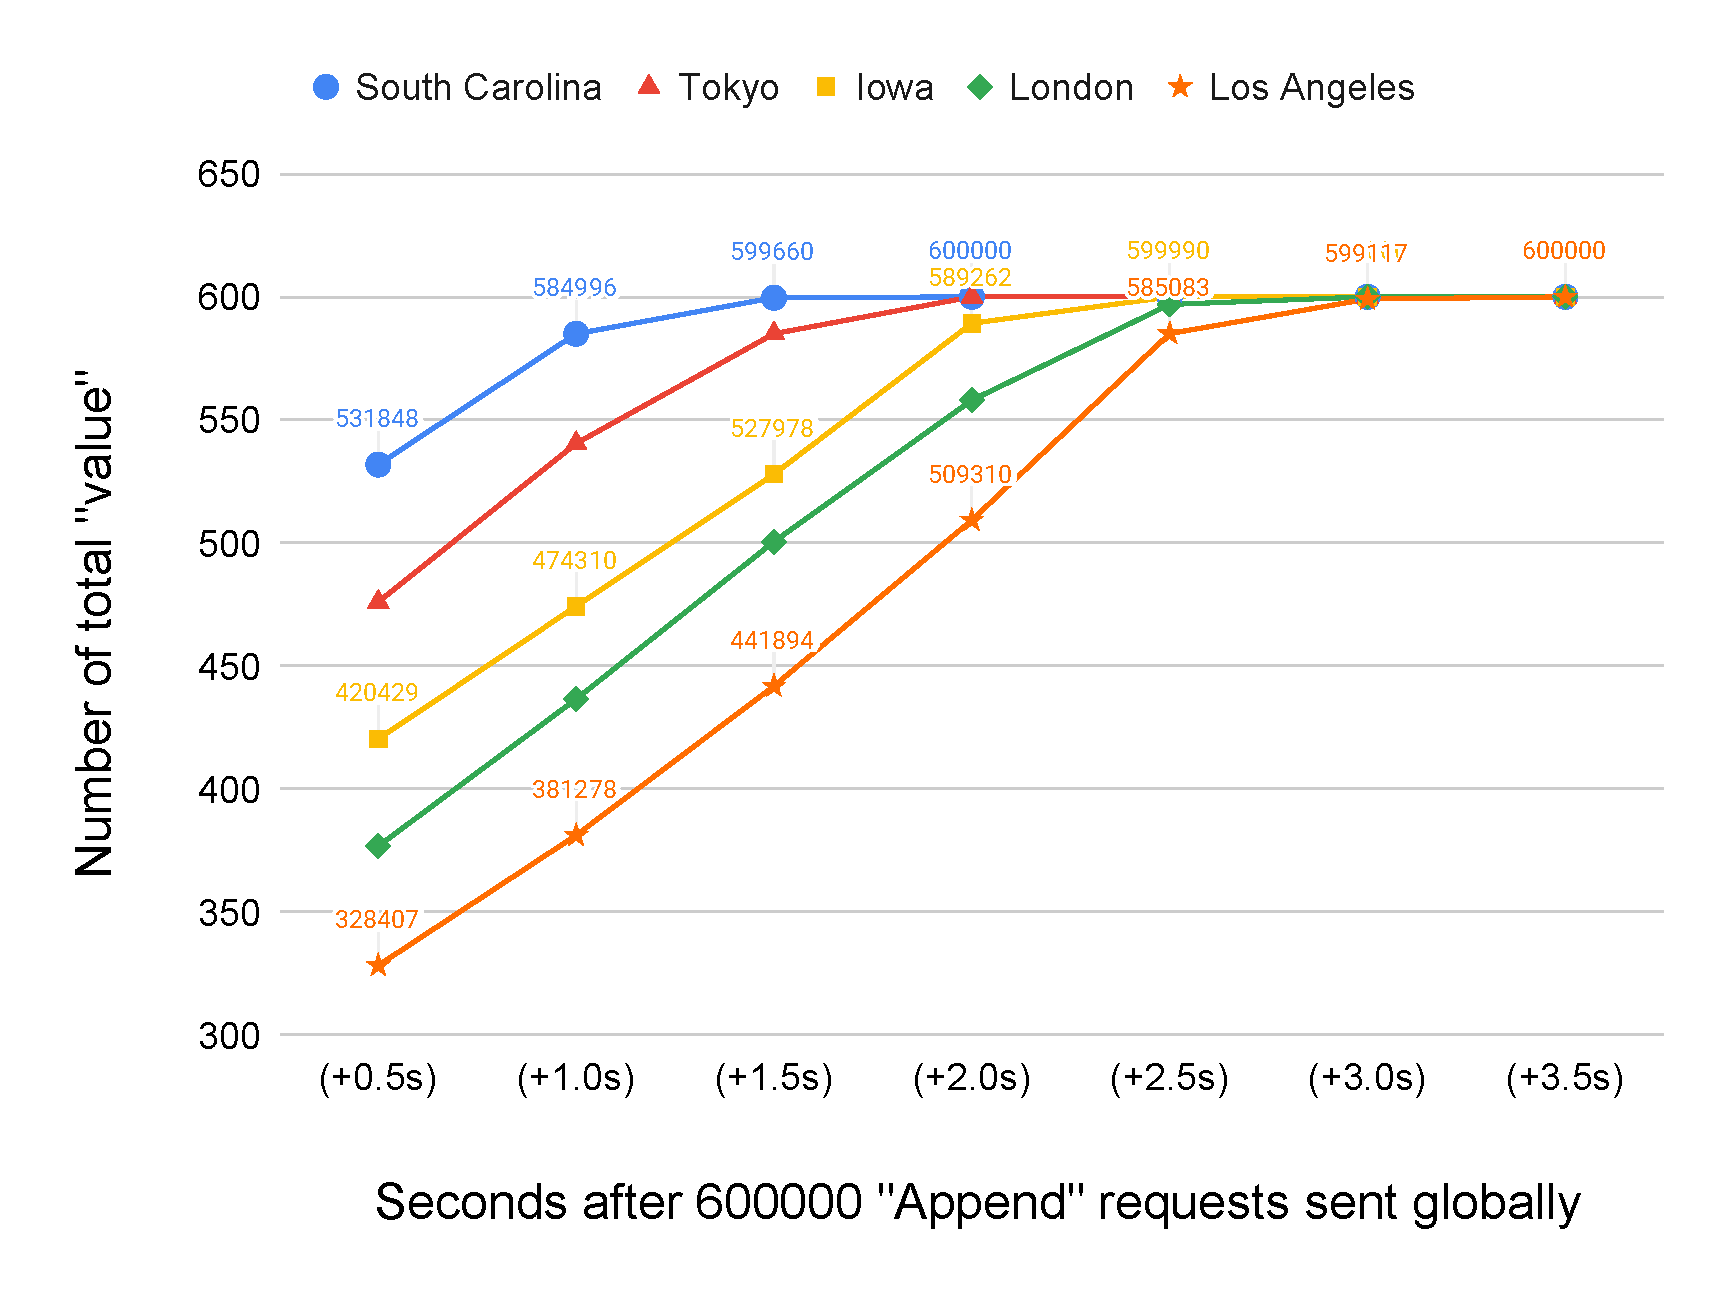
\includegraphics[width=8cm]{figure/consistency.pdf}}
	\subfigure[Get Request Latency.]{\label{fig:g}
		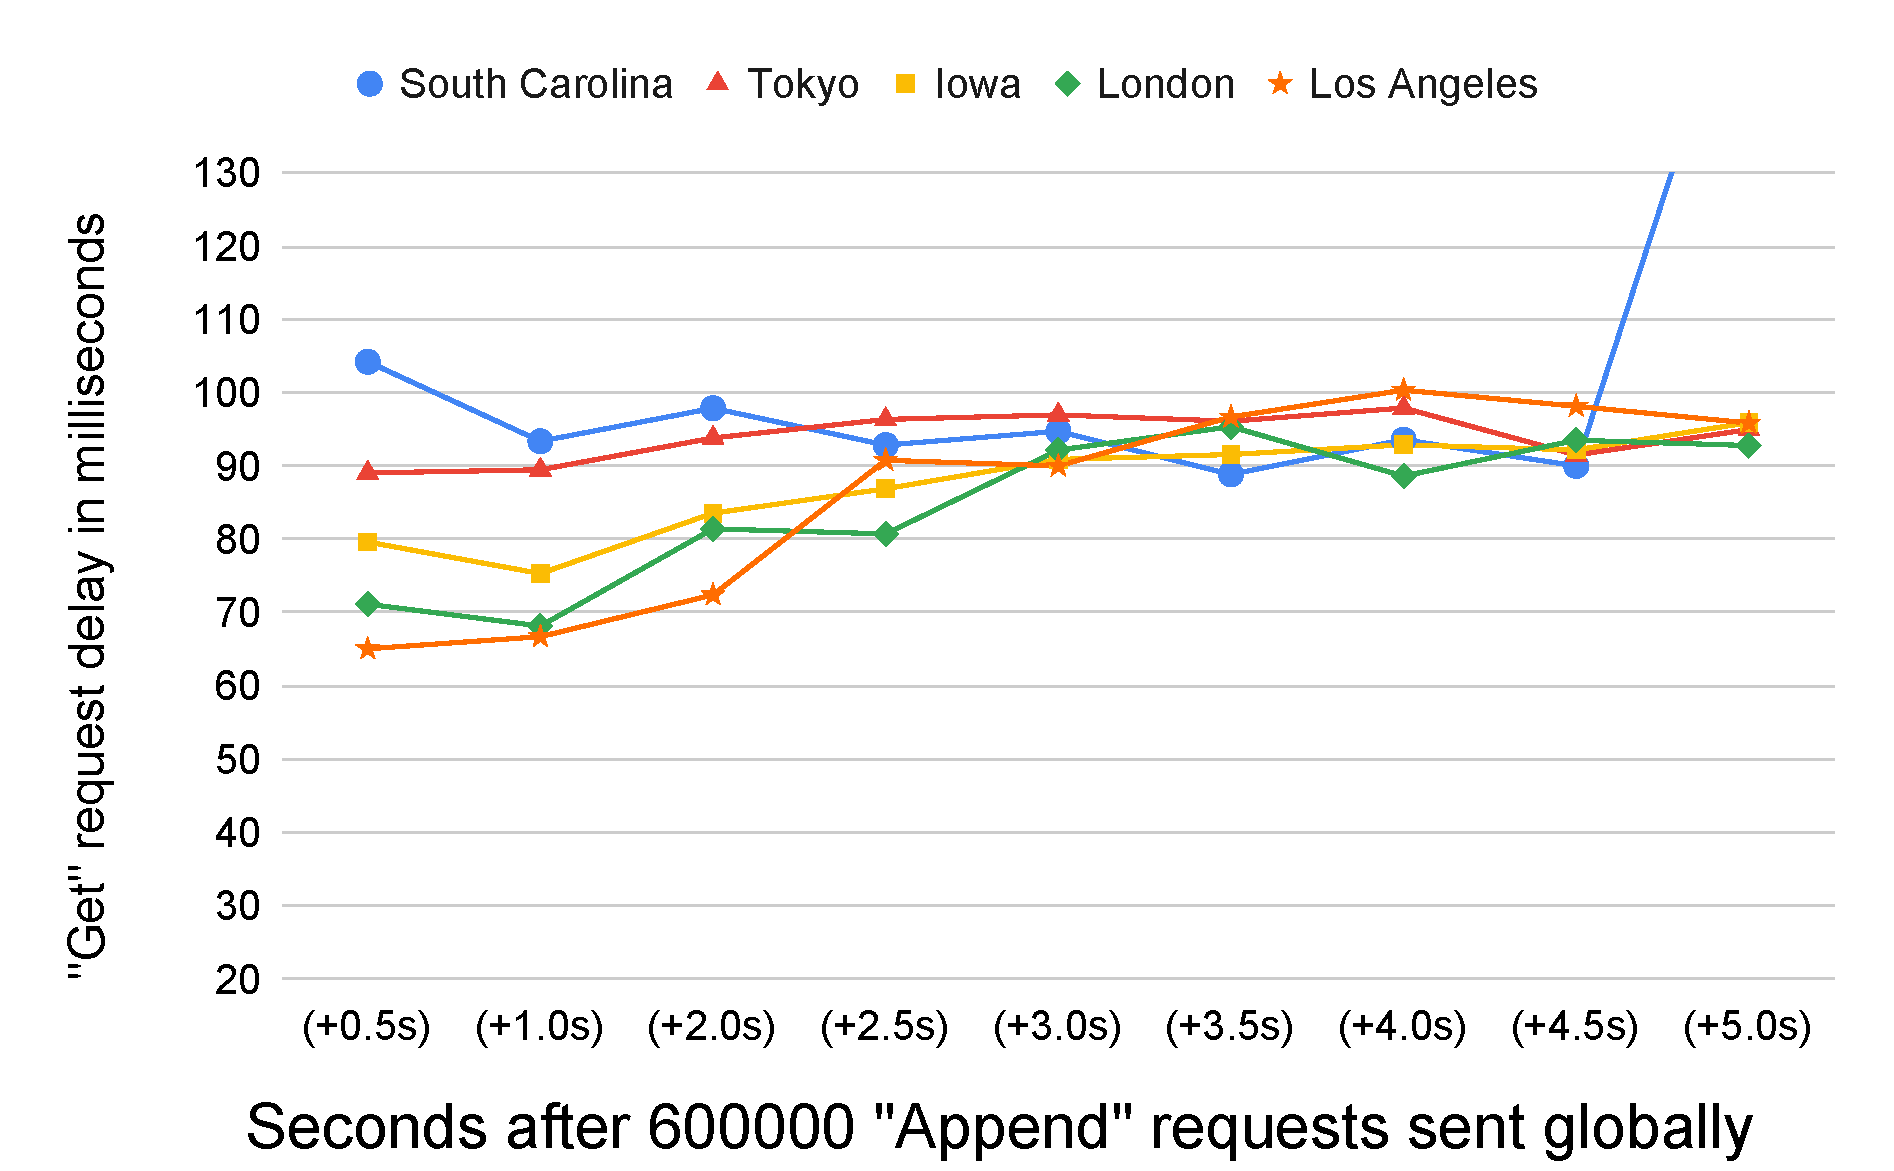
\includegraphics[width=8cm]{figure/GetRequestLatency.pdf}}
\caption{Performance Test Result}
\vspace{-0.4cm}
\label{ConsistencyDelay}
\end{figure}

\subsection{Get Request Performance}
The result of the \texttt{Get} is shown in Figure \ref{ConsistencyDelay}.
Latency starts differently because the Follower held different amount of data.
After 3.5 seconds, the latency of different Followers converged to between 90
milliseconds and 100 milliseconds. Note that the implementation of \texttt{Get}
could be optimized to achieve better performance.

% Get request delay figure
%\begin{figure}[h]
%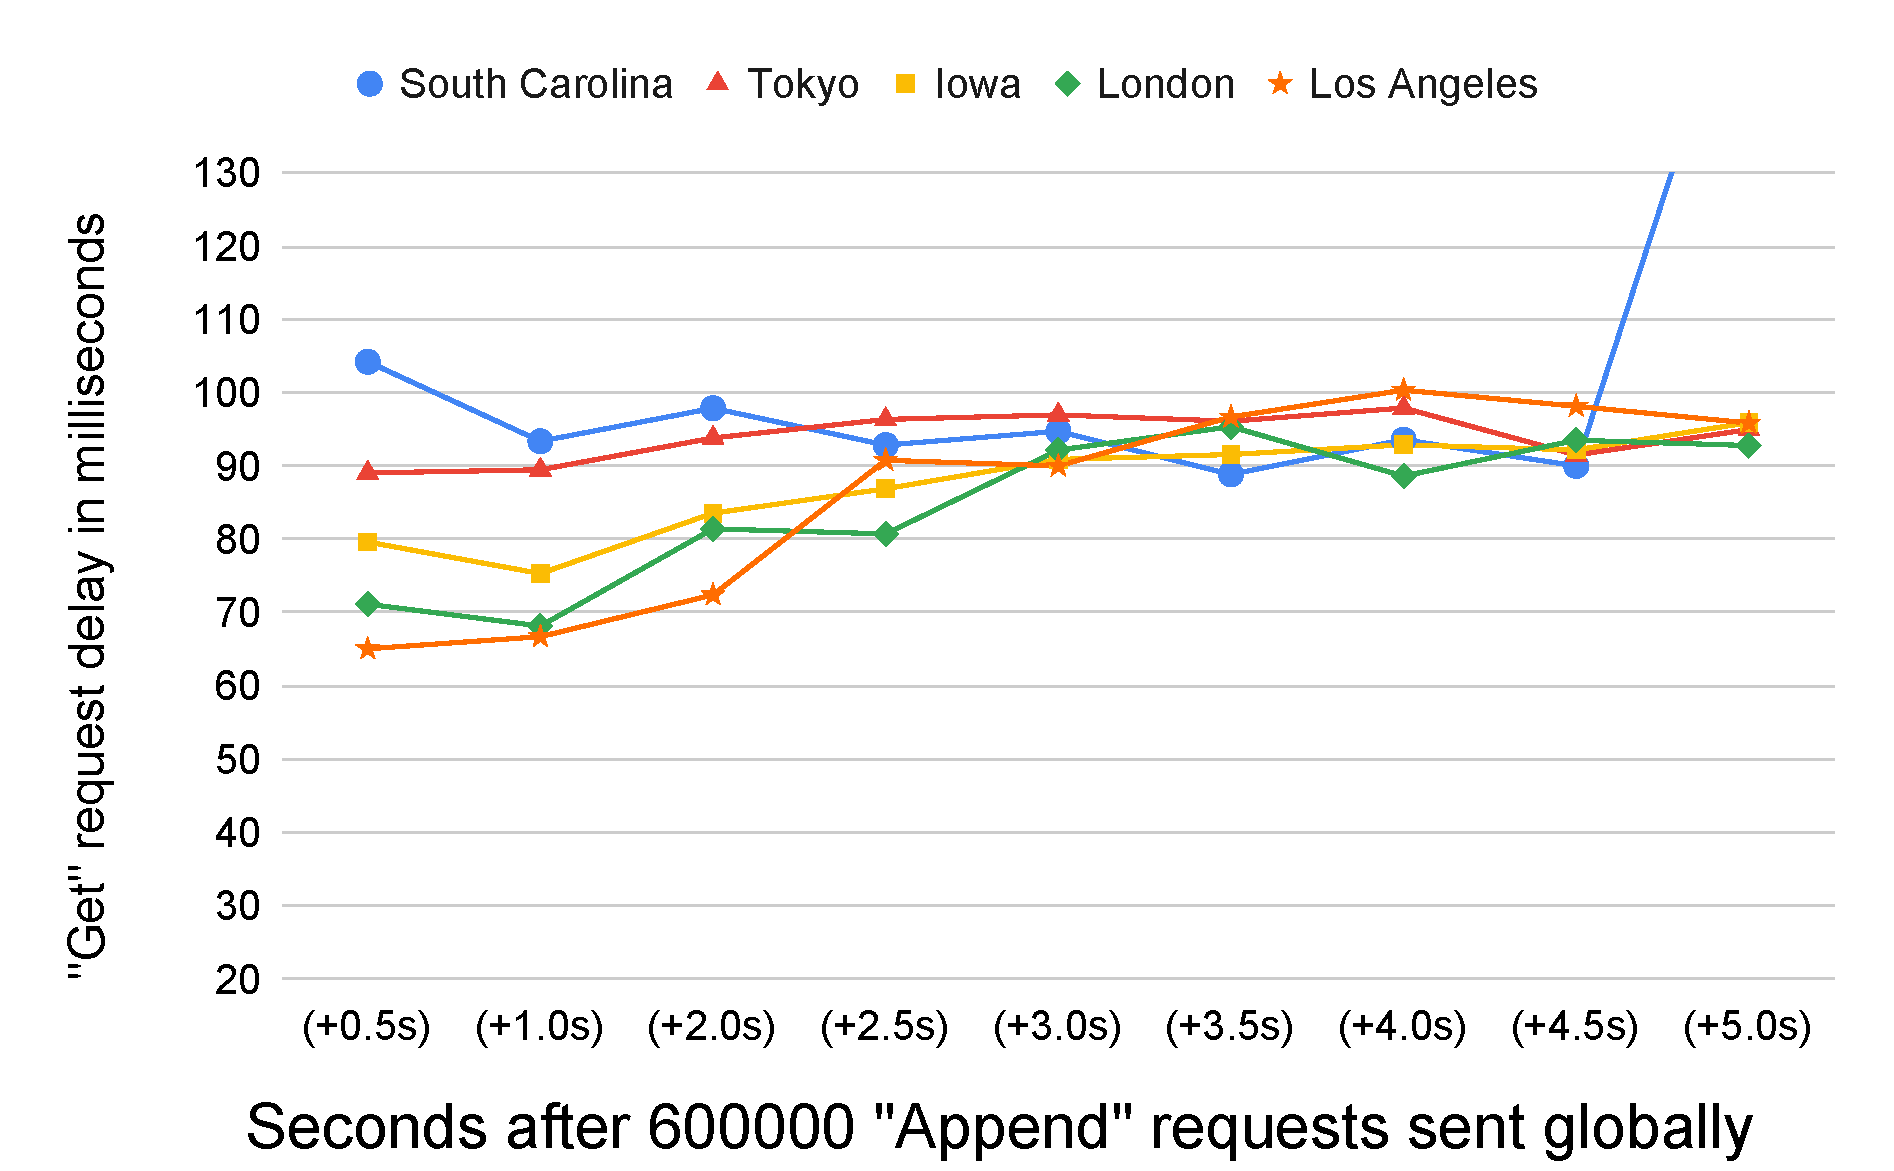
\includegraphics[width=8cm]{figure/GetRequestLatency.pdf}
%\caption{Get Request Latency}
%\label{GetRequestLatency}
%\end{figure}
\vspace{-0.4cm}
\section{Future Work}
We could greatly increase throughput by providing a client library (rather than
a raw GRPC interface) that is aware of the indices or latest index it holds.
This would enable followers to selectively return only the few pieces of data a
client is missing rather than all the data.

To increase fault tolerance, we have discussed making each follower and the
leader their own small cluster of consensus nodes. This would greatly increase
fault tolerance and, while it may complicate the system, would not complicate
clients or the protocols via which nodes communicate.

Lastly, there may be cases where followers fail or are partitioned from their
nearby clients. In these cases, we would like to explore whether clients can
fall back to another follower.
\vspace{-0.3cm}
\section{Conclusions}
We built a datastore to provide low latency and high availability for append-only
data storage. While this work is tailored to a specific set of workloads, there
are numerous applications that can benefit from this approach.

Our system can be used to support distributed services such as distributed
monitoring and chat applications with high performance. Importantly, it exposes
a simple interface allowing for simple clients. We believe that this makes it a
useful tool in building distributed and microservice systems.
\vspace{-0.4cm}
\bibliography{paper} 
\bibliographystyle{ieeetr}

\end{document}
